% !TEX root = ../main.tex

\chapter{Aspirations}
\label{ch:future}

\startcontents[chapters]

\vfill

\begin{alltt}\sffamily
Mid the silence that pants for breath,
when I thought myself at my last gasp,
haine ou de l'ambition et qui se,
the pale motor vessel withdrew its blue breath toward the island's horizon.

As pure and simple as a powder puff,
such also was the ambition of others upon the like occasion,
there was hardly a breath of air stirring,
mon ancien cœur en une aspiration vers la vertu.

After drawing a long breath,
the silver ring she pull'd,
the suitor cried, or force shall drag thee hence.

For wild ambition wings their bold desire,
and with thine agony sobbed out my breath,
I will pull down my barns.
\end{alltt}

\newpage
\minicontents
\spirals


Developing a software product rarely finishes. It is maintained, refactored, repurposed, updated, extended, etc. Especially with creative products, where the functional requirements are more fluid perhaps, it is always tempting to change things. 

For the purpose of this doctoral project, the artefact \url{pata.physics.wtf} is a snapshot of a product in constant motion. The state of the code at the time of submission of this thesis is described in chapter~\ref{ch:implementation}\marginpar{§~\ref{ch:implementation}} and further elaborated on in the \nameref{ch:analysis} chapter\marginpar{§~\ref{ch:analysis}}. But it may very well continue to evolve.

Here, in this chapter I will lay out some of the potential further work for this project. This may continue on a private basis or in a more academic environment. 


\section{Performance}
\label{s:performance}

\paragraph{Startup} 
The website can be slow to load. Currently speed performance was not a priority during development. In fact it is not built for speed from the ground up. Each time the server restarts, the indexing process takes place from scratch (see chapter~\ref{s:setup}\marginpar{§~\ref{s:setup}}). This takes time. Google and other big web search engines do this continuously in the background to keep data up to date. The index\marginpar{§~\ref{s:index}} is currently cached after startup but perhaps preprocessing it and storing it more permanently in a database would help speed up the start. However this may not be necessary, as it only affects the server startup.

\paragraph{Query Response} 
The time it takes from the user entering a query term and the system displaying the results page varies between unnoticable short and impatiently long. This is due to the pataphysicalisation process. This requires calls to external and internal \ac{API}s such as Flickr and WordNet. See analysis on speed issues in table~\ref{tab:percent}\marginpar{\faicon{table}~\ref{tab:percent}}.

\paragraph{Preprocessing Corpora} 
At this point the texts in the corpora consist of almost unedited plaintext (`.txt') files\footnote{For text files downloaded from Project Gutenberg, the Gutenberg specifc copyright notices have been removed to only contain the relevant body of text.} (see chapter~\ref{s:corpora}\marginpar{§~\ref{s:corpora}}). Newlines and whitespace formatting varies, as does language and quality of spelling. Generally, chapter headings, chapter numberings, etc. were left untouched. The Shakespeare corpus contains poetry and plays for example. With the plays, scene information, stage directions, and voice details were kept. This means sentences that appear in the results of the search tool can contain peripheral words such as in this example: ``\ldots Athens and a wood near it ACT I \ldots'' from \textit{A Midsummer Night's Dream} or this example: ``\ldots Exit SHERIFF Our abbeys and our priories shall pay This expedition's charge \ldots'' from \textit{King John}. This could be addressed by preprocessing the individual texts in advance and removing any text that might interfere with the readablility of results.

\paragraph{Image Sizes} 
At the moment images are retrieved at one specified size through the various \ac{API} calls even though they are displayed at various different sizes depending on their location in the image spiral (unless they are displayed as a list). This process could certainly be optimised. Smaller image sizes could be accessed via the \ac{API}s.


\section{Design}
\label{s:designaspi}

\paragraph{Responsive Spirals} 
Currently the image and video spirals (see chapter~\ref{s:imgvid}\marginpar{§~\ref{s:imgvid}}) are fixed size. This means that when the webpage is resized the spiral stays the same size and is left-aligned on the page. Ideally it would be better to scale the spiral with the width of the browser page. This could be achieved using percentage widths, although it would require a lot of work to adapt the current code for the spirals (see chapter~\ref{s:imgspiral}\marginpar{§~\ref{s:imgspiral}}).

\paragraph{Scalable Image Sizes} 
As mentioned above, images are retrieved at one size through the various \ac{API} calls. Because images in the spiral have different sizes according to where in the spiral they are located, they are scaled up or down directly in the \ac{HTML} code. This means that some of the images look distorted and pixelated if they have to be scaled up or down too much.

\paragraph{Square Aspect Ratio} 
Another issue is the aspect ratio of images and videos. For the spiral they need to be square. They are currently distorted as opposed to cropped. It might be possible to specify an option in the \ac{API} calls to only retrieve square images which would help this problem.

\paragraph{Responsive Poems} 
A similar problem to the responsive spirals exists with the display of the Queneau poems. The random poems are centered on the page but the Queneau poems require a lot more formatting and styling to render and currently this is achieved by left-aligning them and having a fixed `absolute' position on the page. Ideally this would also be centered as in the random poems. 

\paragraph{Paginate Results}
For the text-by-source and text-by-algorithm search as well as the image- or video-as-list search results, it may improve the loading speed of the results page to split the results into smaller chunks and display them on several pages instead of one long scrolling page. This is called pagination.

\paragraph{Random Sentences} 
Adding to the source of random sentences used in the top and bottom banner on the website should be an ongoing endeavour. The current list of sentences used is shown in appendix~\ref{s:appsentences}\marginpar{§~\ref{s:appsentences}}.


\section{Text}
\label{s:textfuture}

\paragraph{Result Sentences} 
Currently the way result sentences are retrieved for the text search is based on punctuation (see chapter~\ref{s:ressent}\marginpar{§~\ref{s:ressent}}). This means once a pataphysicalised keyword has been found, the system retrieves up to \num{10} words prior until it reaches a punctuation mark and the same for after. The idea here was to get suitable sentence fragments. This could be changed to rely on \ac{POS} tags for example or simply retrieving complete sentences.

\paragraph{Stopwords}
When the index is created only words that are not considered stopwords are added. We could modify the list of stopwords (see appendix~\ref{s:stopwords}\marginpar{§~\ref{s:stopwords}}) to include a few more uninteresting words. Or we could simply remove everything but nouns for example. This would drastically influence the results produced by the system.

\paragraph{Rhyming Scheme} 
One of the biggest points for future work is to introduce a rhyming scheme for the poetry results. This might involve some more \ac{NLP} during the creation of the index\marginpar{§~\ref{s:index}}. It would make the poems much more readable. This could include pronounciation \ac{POS} tags or other \ac{IPA} like data (for example using an \ac{API} like Wordnik \autocite{Wordnik2016} or a library like \ac{NLTK}). So a word in the index dictionary might contain the following items.

\begin{minted}{text}
  (``tree'': [``l_00'': [24,566,4990], ``s_14'': [234,5943]], ``[tri]'')
\end{minted}

By doing \ac{POS} tagging\marginpar{§~\ref{s:pos}} with pronounciation data, we could retrieve sentences that match the sound of the last word of the previous line for example.


\section{Pataphysicalisation}
\label{s:pataasp}

\paragraph{WordNet}
The vocabulary in WordNet is limited. According to its website \autocite{Princeton2010} it contains \num{117000} `synsets'\footnote{Synonyms---``words that denote the same concept and are interchangeable in many contexts''---are grouped into unordered sets called synsets \autocite{Princeton2010}.} This affects two of my algorithms (namely the Syzygy and Antinomy algorithms). See also discussion in chapter~\ref{s:analsyzygy}\marginpar{§~\ref{s:analsyzygy}}. An option might be to somehow widen the amount of word matches by including different word-types/forms and relationships, such as troponyms, homonyms and heteronyms. Using these could introduce a whole new kind of pataphysical result. 

Homonyms are pronounced the same but mean something else (e.g. `write' and `right'). Heteronyms are words that are spelled the same but have a different meaning (e.g. `close to the edge' and `to close the door'). Homophones are often used to create puns (and remember---puns are syzygys of words), for example ``past your eyes'' and ``pasteurize''. 

\begin{quotation}
   You can tune a guitar, but you can't tuna fish. Unless of course, you play bass. \sourceatright{(attributed to Douglas Adams)}
\end{quotation}

\paragraph{Antinomy}
The antinomy algorithms relies on WordNet's antonyms. A lot of words simply do not have an opposite and no fallback is currently defined. This means a lot of the time the antinomy function will not produce any results. Andrew Dennis implemented the algorithm in the same way, as discussed in chapter~\ref{s:dennis}\marginpar{§~\ref{s:dennis}}. It would be great to come up with a better way of dealing with this concept to ensure results are produced everytime.

\paragraph{Stemming}
Stemming could increase the number of results found by all algorithms (see chapter~\ref{s:nlp}\marginpar{§~\ref{s:nlp}}). A danger of increasing the output of the pataphysicalisation is always that results become more boring. Currently queries such as `clear' and `clearing' are treated as separate entities and would produce different results. Stemming would turn both of these words into the stem `clear' and they would return the same results. Now it becomes immediatly clear (no pun intended) though that this might not always be desirable as just illustrated in this sentence: the root meaning of `clear' can be very different to the meaning of `clearing'.

\paragraph{Queneau's poems}
It would be nice to actually add Queneau's poems \autocite{Queneau1961} into the Faustroll corpus as little easter egg (see chapter~\ref{s:culture}\marginpar{§~\ref{s:culture}}).

\paragraph{Image Algorithms}
\label{s:imgalgoimprovs}
The image and video search currently rely on external \ac{API}s (see chapter~\ref{s:imgvid}\marginpar{§~\ref{s:imgvid}}). One option to approach this in a totally different way would be to write algorithms that analyse and pataphysicalise the actual image or video data themselves. This might involve manipulating histograms or pixel maps.

\paragraph{Maximum Obscurity}
N-grams are a \ac{NLP} technique introduced in chapter~\ref{s:ngrams}\marginpar{§~\ref{s:ngrams}}. The idea is that it allows for prediction of likely word pairs, meaning if the word `sunny' often occurs just before the word `day' in a given training text or corpus then the probability for this particular n-gram is higher than say for `sunny dog'. This can be increased to predict the probability of longer chains of words. One can immediately see the attraction of abusing this to generate pseudo sentences or even of creating a formula similar in nature but for example ranking obscure combinations of words higher than common ones. So for example instead of having a \acf{MLE} (see equation~\ref{eq:mle}\marginpar{$\bm{\Sigma}$~\ref{eq:mle}}) we could have a `Maximum Obscurity Estimation' which returns the highest probabilty for word sequences that happen the rarest.

\paragraph{Pataphysical Entropy}
Similarly, we could play with maximum entropy models as shown in chapter~\ref{s:maxent}\marginpar{§~\ref{s:maxent}} together with \ac{POS} tagging\marginpar{§~\ref{s:pos}} by rigging given probability for tags. There are endless possibilities of abusing these kinds of techniques. This is also very reminiscent of \ac{OULIPO} techniques. 

\paragraph{Grammars}
We could create a whole new language grammar based on pataphysical principles. Examples of using a standard grammar (see chapter~\ref{s:grammars}\marginpar{§~\ref{s:grammars}}) for generating `random' text are as follows\footnote{\autocite{Winter2016,Dada2016,Stribling2016}}.

\begin{adjustwidth}{1cm}{}
\begin{description}[leftmargin=3cm]
  \item[ArtyBollocks] Generates artist statements.
  \item[DadaEngine] A system for generating random text from grammars.
  \item[SciGen] Generates random Computer Science research papers.
\end{description}
\end{adjustwidth}

\paragraph{Uncreativity}
In chapter~\ref{s:csf}\marginpar{§~\ref{s:csf}} I discussed the concepts of uninspiration and aberration by Wiggins and Ritchie \autocite*{Wiggins2006,Ritchie2012} in relation to their \ac{CSF}. We could define a `Pataphysical Search Framework' in the same way. Table~\ref{tab:csf}\marginpar{\faicon{table}~\ref{tab:csf}} shows some of their original definitions for various forms of aberration and uninspiration. Table~\ref{tab:patacsf}\marginpar{\faicon{table}~\ref{tab:patacsf}} then shows some rough ideas about how pataphysical concepts might be defined.

\begin{adjustwidth}{1cm}{}
\begin{description}[leftmargin=2.5cm]
  \item[Clinamen] smallest possible aberration to make the biggest difference
  \item[Antimomy] reachable, abnormal concepts with value
  \item[Anomaly] reachable concepts outside the norm
  \item[Absolute] criteria for value and norm must be perfectly matched
  \item[Syzygy 1] concepts reachable within 3 steps from the query
  \item[Syzygy 2] transformed set of concepts $S_{obj} \rightarrow S^{meta} \rightarrow S'{obj}$
\end{description}
\end{adjustwidth}

This is definitely work in progress and it would be out of the scope of this thesis to elaborate much further.

\begin{table}[!htbp]
\centering
\caption{CSF concept definitions of uncreativity (see chapter~\ref{s:csf})}
\label{tab:csf}
\begin{tabu}{ll}
\toprule
\textbf{Name} & \textbf{Equation} \\
\midrule
Universal set of concepts & $U$ and $X \subseteq U$ \\
Aberration & $B \text{ where } B \notin N_\alpha (X) \ \wedge \ B \neq \emptyset$ \\
Perfect Aberration & $V_\alpha (B) = B$ \\
Productive Aberration & $V_\alpha(B) \neq \emptyset \ \wedge \ \neq B$ \\
Pointless Aberration & $V_\alpha(B) = \emptyset$ \\
Hopeless Uninspiration & $V_\alpha (X) = \emptyset$ \\
Conceptual Uninspiration  & $V_\alpha (N_\alpha (X)) = \emptyset$ \\
Generative Uninspiration  & $elements(A) = \emptyset$ \\
\bottomrule
\end{tabu}
\end{table}

\begin{table}[!htbp]
\centering
\caption[CSF pataphysical concepts]{Possible definitions of pataphysical concepts in terms of the CSF}
\label{tab:patacsf}
\begin{tabu}{XX[5]} 
\toprule
\textbf{Name} & \textbf{Equation} \\
\midrule
Norm & $N_\alpha (X) = \{c \in X \ | \ N(c)> \alpha\} \text{ where } N \in [0,1]^X$ \\
Value & $V_\alpha(X) = \{c \in X \ | \ V(c) > \alpha\} \text{ where } V \in [0,1]^X$ \\
Pata & $P_\alpha(X) = $ \newline $\{c \ | \ c \in(CLI(X)\cup ANT_\alpha(X) \cup SYZ(X) \cup ANO_\alpha(X) \cup ABS(X))\}$ \\
Clinamen & $CLI(X) = \{c \in X \ | \ N_{0.9} (N_{0.1} (c))\}$ \\
Antinomy & $ANT_\alpha(X) = \{c \in X \ | \ V(N_0(c)) > \alpha\}$ \\
Anomaly & $ANO_\alpha(X) = \{c \in X \ | \ N(c)< \alpha\}$ \\
Absolute & $ABS(X) = \{c \in X \ | \ V_1 (N_1 (X)) \neq \emptyset\}$ \\
Syzygy 1 & $SYZ(query) = \bigcup_{n=0}^{3} elements(Q(N,V)^n (query))$ \\
Syzygy 2 & $SYZ(X) = S'(X) \text{ where } S_{obj} \rightarrow S^{meta} \rightarrow S'{obj}$ \\
\bottomrule
\end{tabu}
\end{table}


\section{Extensions}
\label{s:extensions}

\paragraph{Additional APIs} 
Currently 5 \ac{API}s\footnote{Flickr, Getty, Bing, MicrosoftTranslator and YouTube} are used in \url{pata.physics.wtf}. This could be increased to include more varied sources of data. Sites like Flickr are heavily based on user tags (`folksonomies') which can be unreliable and a bit random at times. Possible additional \ac{API}s to consider would be Instagram, Imgur, Facebook, Google Image Search, DeviantArt, Pinterest, Vimeo, Twitter, SoundCloud, etc.

\paragraph{Web Search} 
The use of \ac{API}s could also include web search results rather than just images and videos. This would need its own interface section and a suitable display style for the results. The biggest problem for this are \ac{API} limitations as mentioned in chapter~\ref{s:apis}\marginpar{§~\ref{s:apis}}. Alternatively a ready-made index or crawl could be used but these are typically many terrabytes in size and have a cost attached. Crawling the web myself is not an option due to the computational power, time and space required to do so.

\paragraph{Additional Algorithms} 
It would be nice to implement some more algorithms for the search tool. This could include the two additional algorithms suggested by Andrew Dennis (see chapter~\ref{s:dennis}\marginpar{§~\ref{s:dennis}}) or developing more of my own. This could involve implementing some of the other pataphysical principles, such as equivalence or anomaly. Or it could consist of implementing some of the more famous \ac{OULIPO} techniques. The repertoire of them is huge (see tables~\ref{tab:oulipo1} and \ref{tab:oulipo2}\marginpar{\faicon{table}~\ref{tab:oulipo1} \& \ref{tab:oulipo2}}).

\paragraph{Custom API}
Finally, it would be great to develop a custom \ac{API} for the algorithms of \url{pata.physics.wtf}. This would allow other people to use the search remotely without going through the interface and to use the results as they want. This would have been beneficial for the Digital Opera project\marginpar{§~\ref{s:opera}} and certainly for other researchers/developers like Andrew Dennis\marginpar{§~\ref{s:dennis}}.


\section{User Testing}

\paragraph{Focus Group}
It might be interesting to look at opinions of various people (general public and experts) about the interpretation/evaluation framework. This could be done by asking them to provide their own definition of computer creativity and then to analyse and evaluate a product (such as \url{pata.physics.wtf}) according to their own criteria. Then follow this up by getting the same people to use my proposed framework\marginpar{§~\ref{s:framework}} to compare the results. This would include asking them about whether or not they thought that using the framework was beneficial to them or confusing.

\paragraph{Eye-Tracking}
To study the effects of using different styles of presenting the same results, an eye-tracking experiment could be done. This would involve setting up participants with the necessary equipment and then introduce them to \url{pata.physics.wtf} and moniter their eye movements as they navigate the site. This could also provide details about how long users spend on each results page, what kind of style of results they prefer, etc. Some may prefer image or video search over the text search while others may not be interested in that at all. Generally of course one has to take into account that this is a creative piece of work and not everybody will like it. It is purposefully purposeless and highly subjective, so user feedback may not provide unbiased and useful results.


\section{Audio}
\label{s:audio}

Audio search completes the spectrum of pataphysical search tools. Being outside the scope of this doctoral project, it is left open for potential future work, but I want to elaborate a little bit on the significant connection between pataphysics and music.


\subsection{History}
\label{s:history}

Andrew Hugill argues that ``pataphysics has become a byword for experimentation and left-of-field work'' in digital and electronic music \autocite*{Hugill2012}. He lists several artists \footnote{Experimental German electronica band \textit{Farmer’s Manual}, Paul D. Miller, better known as \textit{DJ Spooky}, American ambient experimental musician \textit{Faustroll}, Australian-Sri Lankan rapper \textit{Pataphysics}, electronic music artist \textit{Tomoroh Hidari} a.k.a. Oliver Stummer, American `avant-garage' rock group \textit{Pere Ubu}, and English avant-garde musician, artist and occultist \textit{Genesis Breyer P-Orridge}.} as examples of pataphysical musicians but highlights a few names in particular as key figures in this genre. 

\emph{John Cage} was an American composer, musician, writer, philosopher, and artist (1912---1992). He is often associated with the avant-garde movement (his close friend Marcel Duchamp is also famous for his involvment in this), which itself can be said to be related to Dada, \ac{OULIPO}, and of course Pataphysics (see \autocite{Hugill2012}). Pataphysical influences abound in Cage's work and words (although he appears to be an unconscious rather than conscious Pataphysician). For example he explained he ``was shocked at college to see one hundred of my classmates in the library all reading copies of the same book. Instead of doing as they did, I went into the stacks and read the first book written by an author whose name began with Z'' \autocite{Cage1989}, an act of antinomy. A very Oulipian approach to composition comes from his use of chance: he developed ``complicated composing means using I Ching chance operations, making my responsibility that of asking questions instead of making choices'', in fact he said his work ``became an exploration of non‑intention'' \autocite*{Cage1989}. This also resembles the chance swerve of the clinamen in pataphysics.

\begin{quotation}
  [\ldots] all of the incidents were critical, all of the people influenced me, everything that happened and that is still happening influences me. \sourceatright{\autocite{Cage1989}}
\end{quotation}

Cage was also influenced by Zen Buddhism, which he called a mixture of ``humor, intransigence, and detachment''\footnote{He also refers to his friend Duchamp here: ``[Zen] makes me think of Marcel Duchamp, though for him we would have to add the erotic''.} \autocite*{Cage1989}. The antinomy and \ac{OULIPO} influences are strongest in Cage's famous \textit{4$\prime$33$\prime\prime$} piece from 1952. Hugill compares this to an earlier, similar work by Alphonse Allais from 1884 called \textit{Marche funèbre composée pour les funérailles d’un grand homme sourd} (`Funeral March for the Obsequies of a Large Deaf Man') \autocite*{Hugill2012}. \textit{4$\prime$33$\prime\prime$} was inspired by Rauschenberg's white paintings \autocite*{Rauschenberg1951} and ``in the anechoic chamber at Harvard University [Cage] heard that silence was not the absence of sound but was the unintended operation of [his] nervous system and the circulation of [his] blood'' \autocite{Cage1989}. He called the composition his `silent piece' and it consist of three movements, during which performers are instructed to \emph{not} play their instruments\footnote{The John Cage Foundation also released an app called 4$\prime$33$\prime\prime$ which allows users to listen, record and share ambient soundscapes \autocite{Cage2016}.}.

The connection to pataphysics is less obscure in \emph{the Beatles}. The lyrics of \textit{Maxwell's Silver Hammer} go: 

\begin{quotation}
  Joan was quizzical\\
  studied pataphysical\\
  science in the home.

  [\ldots]

  Bang! Bang! Maxwell's silver hammer\\
  came down upon her head.\\
  Bang! Bang! Maxwell's silver hammer\\
  made sure that she was dead.

  [\ldots]\sourceatright{\autocite{LennonMcCartney1969}}
\end{quotation}

This clearly references pataphysics and Ubu's \textit{Debraining song}. Hugill explains that Maxwell's ``silver hammer repeatedly comes down `bang, bang' upon the heads of those who, in their normality, have offended him in various ways, and `makes sure that they are dead.' Just like the `Chanson du décervelage,' the Beatles’ tune is reminiscent of music-hall: childishly simple and ironically joyous'' \autocite*{Hugill2012}. 

Apparently McCartney’s interest in pataphysics started with the radio broadcast of Jarry's \textit{Ubu Cuckolded} in 1966 \autocite[Miles 1997, as cited in][]{Hugill2012}, which he much later developed into a radio show called \textit{Oobu Joobu} for an American network in 1995 \autocite{Hugill2012}. This is also around the time Lennon met Ono, who was involved with the avant-garde neo-Dada artist group Fluxus and may very well have been aware of Jarry and pataphysics.

\emph{Frank Zappa} is considered a major figure in pataphysical music, ``most of whose recorded output may be viewed as a pataphysical legacy, albeit not explicitly labeled as such'' \autocite{Hugill2012}. His 1974 album \textit{Apostrophe(')} \autocite*{Zappa1974} perhaps directly references Jarry's spelling of ``'pataphysics'' with the perplexing leading apostrophe (see page~\pageref{s:apostrophe}). The connection is certainly made in reverse: in a book review of \textit{Faustroll}, Nathan Gaddis cites a Zappa lyric from the song \textit{Stink-Foot} from said album (``the crux of the biscuit is the Apostrophe(')''):

\begin{quotation}
  What precisely is the status of the Apostrophe in ‘pataphysics? The answer should be obvious but then when one reads the sacred texts closely it becomes suddenly and little by little not quite so clear that there is any kind of apo’consistancy. Perhaps it is only in so far as it remains \emph{the crux of the biscuit}. \sourceatright{\autocite[][emphasis added]{Gaddis2014}}
\end{quotation}

\emph{Gavin Bryars} is an English composer and musician and holds the title of `Transcendent Satrap', the highest position attainable in the French Collège de {'}Pataphysique \autocite{Bryars2010}. In 1972 he wrote the ``musical equivalent of a work of conceptual art'' \autocite*{Bryars2009} entitled \textit{The Sinking of the Titanic}, which ``explicitly set out to give a pataphysical account of the tragedy'' \autocite{Hugill2012}.

\begin{quotation}
  The piece included fragments of interviews with a survivor, Morse signals played on woodblocks, references to the different bagpipe players on the ship (one Irish, one Scottish), miscellaneous sound effects relating to descriptions given by survivors of the sound of the iceberg’s impact, and other `found materials.' The `imaginary solution' that provided the most overtly pataphysical aspect of the piece, however, was the prolongation of the hymn tune `Autumn' that was famously played by the ship’s band, recorded underwater. \sourceatright{\autocite{Hugill2012}}
\end{quotation}

English minimalist and experimental composer \emph{John White}\ published (among others) with the same label as Bryars above---Brian Eno's Obscure Records \autocite{UbuWeb}\footnote{It is worth exploring the UbuWeb sound archive found at \url{http://www.ubuweb.com/sound/}. It contains tracks by various artists related to pataphysics or Jarry in one way or another, such as Appolinaire, Baudrillard, Bök, Borges, Breton, Cage, Dalí, Duchamp, Fluxus, Queneau, Satie, and lots more. The archive also contains two collections of pataphysical recordings \autocite{UbuWebUseless, UbuWebPata}.}. His music ``is generally characterized by the kind of ironical humor and references to found material that typify a certain kind of pataphysical art'' \autocite{Hugill2012}. In 2014, he and his work were subject of a double edition journal of the London Institute of Pataphysics \autocite{Smith2014, White2014}, so it is perhaps not surprising that Hugill calls him their ``composer in residence'' \autocite{Hugill2012}. 

Similarly, the progressive rock band \emph{Soft Machine} was considered, ``somewhat to their surprise, the `official orchestra of the College of Pataphysics' in the late 1960s'' \autocite{Hugill2012}. Robert Wyatt, the band's drummer and singer, ``had the spiral {'}pataphysics logo painted on his bass drum, and still has a copy of Jarry's writing on his bookshelf today'' \autocite{ODair2014}.

\begin{quotation}
  Wyatt was introduced to {'}pataphysics in 1967, when Soft Machine---already established, alongside Pink Floyd, as darlings of the London underground scene, and about to tour the States with the Jimi Hendrix Experience---performed a live soundtrack to Ubu Enchaîné at the Edinburgh Festival. By the time of their second album, Wyatt was introducing the band as ``the official orchestra of the College of {'}Pataphysics,'' going on to prove these credentials by singing the letters of the alphabet in reverse. This was a clear echo of Jarry himself, who had advocated the backwards meal, commencing with brandy and ending with soup.

  Always interested in modernism, it is no surprise that Wyatt felt a broad affinity with the Frenchman, whose Ubu Roi had arguably kicked off the whole movement. In particular, Wyatt shares his interest in the ambiguity of language and his emphasis on childhood memory: the grotesque character of Ubu was modeled on Jarry's unpopular physics teacher, Monsieur Hébert. Jarry's habit of turning up to the opera wearing a paper shirt adorned with painted black tie also predates Wyatt's trademark stage outfit---a jacket drawn onto his naked torso in crayon---by over half a century.
  
  [\ldots]

  In terms of his music, the influence of what Wyatt refers to in emails as ``Patafizzix'' is perhaps most obvious in ``Signed Curtain'', a meta-ballad he recorded shortly after leaving Soft Machine. ``This is the first verse, this is the first verse,'' it begins, and continues in similarly self-referential fashion: ``this is the chorus or perhaps it's the bridge\ldots'' And when Wyatt sang on a song for composer John Greaves' 1996 album Songs, he finally got his chance to deliver the line: ``Peel's foe, not a set animal, laminates a tone of sleep.'' It is, surely, the longest grammatically correct palindrome in popular music---and it could have come straight from Jarry's pen.
  \sourceatright{\autocite{ODair2014}}
\end{quotation}

Another musician who could be considered pataphysical (conscious or unconscious) is \emph{Captain Beefheart}, who was friends with Frank Zappa and admired by Paul McCartney and John Lennon \autocite{Hermes2010}. His work is associated with jazz, experimentalism and avant-garde among others. In fact, jazz, and specifically free improvisation, is considered a ``stronghold of pataphysical influence'' \autocite{Hugill2012}. \emph{Reverend Fred Lane}, for example, released an album entitled \textit{Raudelunas ’Pataphysical Revue} in 2002.

German comedian, jazz musician, multi-instrumentalist and actor Helge Schneider (``High Priest of pure idiocy'' \autocite{Bolz1997}) might also be considered a pataphysician, although it is unclear whether or not he is aware of it. His humor is often described as dada-esque, absurd and highly focused on improvisation.

\begin{quotation}
  Nonsense is the point of constantly questioning the norms which man has imposed upon himself, to turn them upside down, or even to change them. Nonsense fights what makes sense in a humorous way.\footnote{Original German: ``Unsinn hat den Sinn, die Normen, die der Mensch sich selber auferlegt hat, immer wieder in Frage zu stellen, auf den Kopf zu stellen, oder sogar zu verändern. Unsinn bekämpft das, was Sinn macht auf humorige Weise.''}
  \sourceatright{\autocite[Helge Schneider, in][(translated by Google)]{Bos2009}}
\end{quotation}

Perhaps the most obvious link between pataphysics and music is the \emph{OUMUPO}; an offshoot of the \ac{OULIPO}\marginpar{§~\ref{s:patalipo}}, which itself was originally part of the French College of Pataphysics. Members include Gavin Bryars and Andrew Hugill. 

\begin{quotation}
  mathematics is the link between literature and music, and music is what poetry aspires to \sourceatright{\autocite{Motte2007}}
\end{quotation}

Last but not least, there is of course Andrew Hugill himself (his book on pataphysics is a key text cited extensively in this thesis \autocite[see][]{Hugill2012}), who composed several pataphysical pieces such as the \textit{Catalogue de Grenouilles} \autocite{Hugill1987} \autocite[see][for a full catalogue of his work]{Hugill2015}. In 2007 he released an album called \textit{the {'}pataphysical piano: the sound and silences of Andrew Hugill} \autocite{Hugill2007}

\begin{quotation}
  Although Jarry's {'}pataphysics is characterised by a certain anarchic euphoria, the collection of pieces on this album generally reflect the more studious and imperturbable aspects of {'}pataphysics since Jarry. They nevertheless contain both the subterranean humour and ironic mystery that are common to the science. They are ``imaginary solutions'' to the problem that faces anybody who wishes to write for piano: how to create something that has not already been created for this instrument, which has been comprehensively explored by previous generations. The album therefore often makes reference to existing music that sits at the edges of piano repertoire, as well as applying unusual compositional techniques and constraints, or adding electroacoustic sounds, in its search for something exceptional. The piano is monolithic. \sourceatright{\autocite{Hugill2007a}}
\end{quotation}


\subsection{Potential}
\label{s:potential}

In relation to \url{pata.physics.wtf}, there is a lot of potential in music and audio, with its research divided into three categories: manipulation, search and composition. 

\subsubsection{Manipulation}

Within the manipluation category, (different representations of) sounds are pataphysicalised directly. There are several approaches to this, such as making changes to sound wave forms (an antinomy pataphysicalisation for example could be to invert a sound wave, i.e. where there was silence there is now noise and vice versa). These manipulations could be applied to specific sections only or the complete sound wave. This kind of manipluation could also be applied to musical scores. Changes might also happen in given compositions of music of multiple instruments (as opposed to pataphysicalising the composition process itself which is covered in section~\ref{s:composition}\marginpar{§~\ref{s:composition}}).

\begin{figure}[!htbp]
\centering
  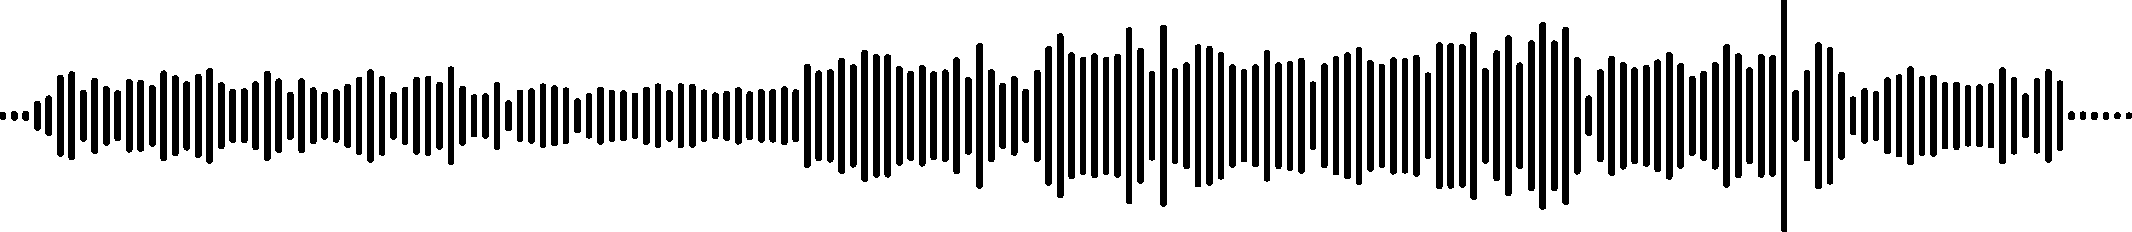
\includegraphics[width=\linewidth]{simplewave.pdf}
\caption{Sound wave}
\end{figure}


- change pitch, compressing?, change of wave form/type (from sine wave to square wave), MIDI,  




The Web Audio API does ``include the capabilities found in modern game audio engines as well as some of the mixing, processing, and filtering tasks that are found in modern desktop audio production applications'' \autocite{Adenot2017}.

an example of using this API to synthesise sounds is described by Misuary \autocite{Misuary2016}



\autocite{soundcloud}




\subsubsection{Search}

- folksonomy tag search (APIs)


\subsubsection{Composition}
\label{s:composition}

- pata constraints to composition




\section{From the Aspirations to Paris by Sea}

\begin{figure}[!htb]
\centering
  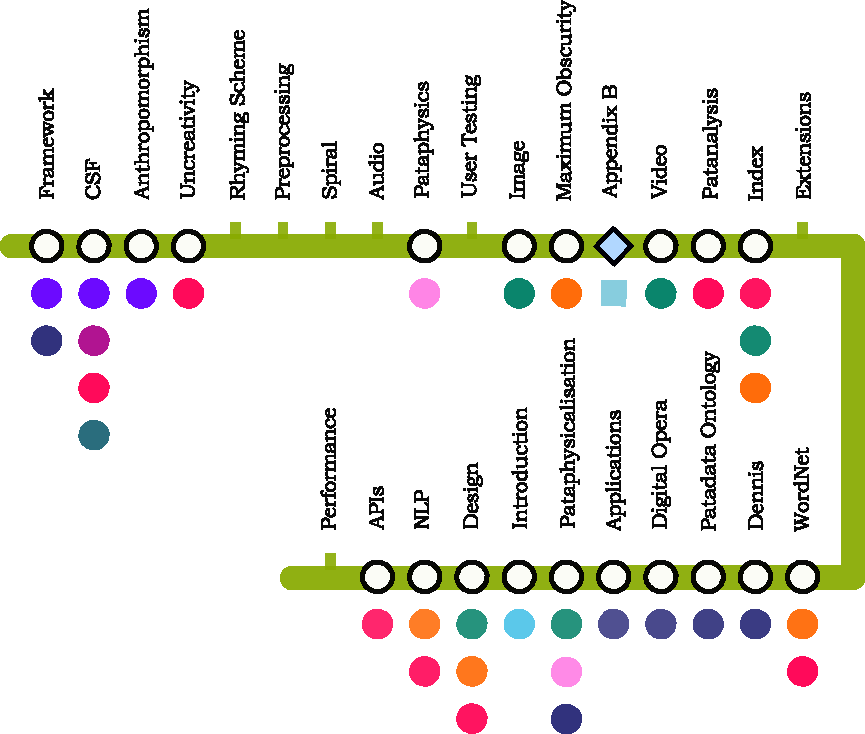
\includegraphics{aspi.pdf}
\end{figure}



\begin{figure}[!htb]
\centering
  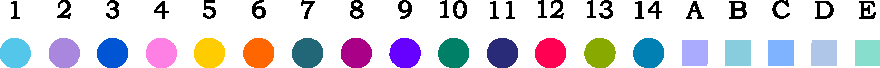
\includegraphics[width=\textwidth]{legend.pdf}
\end{figure}

\stopcontents[chapters]
